\documentclass[tikz]{standalone}
\usepackage{pgfplots}
\pgfplotsset{compat=1.15}
\usepackage{mathrsfs}
\usetikzlibrary{arrows,calc}
\usepackage{tkz-euclide}
\pagestyle{empty}

\definecolor{AngleClr}{rgb}{0,0.39215686274509803,0}
\definecolor{ShapeClr}{rgb}{0.6,0.2,0}
\definecolor{SquareClr}{RGB}{250, 248, 217}

\begin{document}

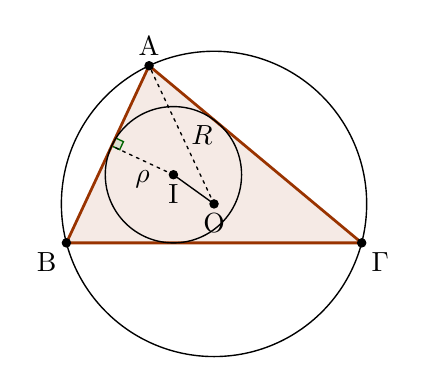
\begin{tikzpicture}[scale=.75]
\tkzSetUpLine[line width=1pt,color=black]
\tkzSetUpPoint[fill=black]

\tkzDefPoints{0/0/B,1.4/3/A,5/0/C}

\tkzDefTriangleCenter[circum](A,B,C) \tkzGetPoint{O}
\tkzDefTriangleCenter[in](A,B,C) \tkzGetPoint{I}

\tkzDefPointBy[projection=onto A--B](I)\tkzGetPoint{IC}

\tkzInterLC(A,I)(O,A) \tkzGetPoints{ZZ}{D}
\tkzInterLC(D,O)(O,A) \tkzGetPoints{E}{ZZ}

\tkzFillPolygon[fill=ShapeClr,fill opacity=0.1](A,B,C)
\tkzMarkRightAngle[line width=0.5pt, size=.15,color=AngleClr,fill=AngleClr,fill opacity=0.1](I,IC,A)

\tkzDrawPolygon[color=ShapeClr](A,B,C)

\tkzDrawPoints[size=3](A,B,C,I,O)

\tkzDrawSegments[line width=0.5pt,color=black,dashed,dash pattern=on 1pt off 1.75pt](I,IC O,A)
\tkzDrawSegments[line width=0.5pt,color=black](O,I)


\tkzDrawCircles[line width=0.5pt,color=black](O,A I,IC)

\tkzLabelPoint[above](A){$\rm A$}
\tkzLabelPoint[below left](B){$\rm B$}
\tkzLabelPoint[below right](C){$\rm \Gamma$}
\tkzLabelPoint[below](O){$\rm O$}
\tkzLabelPoint[below](I){$\rm I$}

\tkzLabelSegment[below](I,IC){$\rho$}
\tkzLabelSegment[right](O,A){$R$}

\end{tikzpicture}

\end{document}
